\documentclass[ignorenonframetext,]{beamer}
\setbeamertemplate{caption}[numbered]
\setbeamertemplate{caption label separator}{: }
\setbeamercolor{caption name}{fg=normal text.fg}
\beamertemplatenavigationsymbolsempty
\usepackage{lmodern}
\usepackage{amssymb,amsmath}
\usepackage{ifxetex,ifluatex}
\usepackage{fixltx2e} % provides \textsubscript
\ifnum 0\ifxetex 1\fi\ifluatex 1\fi=0 % if pdftex
  \usepackage[T1]{fontenc}
  \usepackage[utf8]{inputenc}
\else % if luatex or xelatex
  \ifxetex
    \usepackage{mathspec}
  \else
    \usepackage{fontspec}
  \fi
  \defaultfontfeatures{Ligatures=TeX,Scale=MatchLowercase}
\fi
\usetheme[]{AnnArbor}
\usecolortheme{dolphin}
\usefonttheme{professionalfonts}
% use upquote if available, for straight quotes in verbatim environments
\IfFileExists{upquote.sty}{\usepackage{upquote}}{}
% use microtype if available
\IfFileExists{microtype.sty}{%
\usepackage{microtype}
\UseMicrotypeSet[protrusion]{basicmath} % disable protrusion for tt fonts
}{}
\newif\ifbibliography
\hypersetup{
            pdftitle={Quantitative neuroimaging with ANTs},
            pdfauthor={Nick Tustison},
            pdfborder={0 0 0},
            breaklinks=true}
\urlstyle{same}  % don't use monospace font for urls
\usepackage{color}
\usepackage{fancyvrb}
\newcommand{\VerbBar}{|}
\newcommand{\VERB}{\Verb[commandchars=\\\{\}]}
\DefineVerbatimEnvironment{Highlighting}{Verbatim}{commandchars=\\\{\}}
% Add ',fontsize=\small' for more characters per line
\usepackage{framed}
\definecolor{shadecolor}{RGB}{248,248,248}
\newenvironment{Shaded}{\begin{snugshade}}{\end{snugshade}}
\newcommand{\KeywordTok}[1]{\textcolor[rgb]{0.13,0.29,0.53}{\textbf{#1}}}
\newcommand{\DataTypeTok}[1]{\textcolor[rgb]{0.13,0.29,0.53}{#1}}
\newcommand{\DecValTok}[1]{\textcolor[rgb]{0.00,0.00,0.81}{#1}}
\newcommand{\BaseNTok}[1]{\textcolor[rgb]{0.00,0.00,0.81}{#1}}
\newcommand{\FloatTok}[1]{\textcolor[rgb]{0.00,0.00,0.81}{#1}}
\newcommand{\ConstantTok}[1]{\textcolor[rgb]{0.00,0.00,0.00}{#1}}
\newcommand{\CharTok}[1]{\textcolor[rgb]{0.31,0.60,0.02}{#1}}
\newcommand{\SpecialCharTok}[1]{\textcolor[rgb]{0.00,0.00,0.00}{#1}}
\newcommand{\StringTok}[1]{\textcolor[rgb]{0.31,0.60,0.02}{#1}}
\newcommand{\VerbatimStringTok}[1]{\textcolor[rgb]{0.31,0.60,0.02}{#1}}
\newcommand{\SpecialStringTok}[1]{\textcolor[rgb]{0.31,0.60,0.02}{#1}}
\newcommand{\ImportTok}[1]{#1}
\newcommand{\CommentTok}[1]{\textcolor[rgb]{0.56,0.35,0.01}{\textit{#1}}}
\newcommand{\DocumentationTok}[1]{\textcolor[rgb]{0.56,0.35,0.01}{\textbf{\textit{#1}}}}
\newcommand{\AnnotationTok}[1]{\textcolor[rgb]{0.56,0.35,0.01}{\textbf{\textit{#1}}}}
\newcommand{\CommentVarTok}[1]{\textcolor[rgb]{0.56,0.35,0.01}{\textbf{\textit{#1}}}}
\newcommand{\OtherTok}[1]{\textcolor[rgb]{0.56,0.35,0.01}{#1}}
\newcommand{\FunctionTok}[1]{\textcolor[rgb]{0.00,0.00,0.00}{#1}}
\newcommand{\VariableTok}[1]{\textcolor[rgb]{0.00,0.00,0.00}{#1}}
\newcommand{\ControlFlowTok}[1]{\textcolor[rgb]{0.13,0.29,0.53}{\textbf{#1}}}
\newcommand{\OperatorTok}[1]{\textcolor[rgb]{0.81,0.36,0.00}{\textbf{#1}}}
\newcommand{\BuiltInTok}[1]{#1}
\newcommand{\ExtensionTok}[1]{#1}
\newcommand{\PreprocessorTok}[1]{\textcolor[rgb]{0.56,0.35,0.01}{\textit{#1}}}
\newcommand{\AttributeTok}[1]{\textcolor[rgb]{0.77,0.63,0.00}{#1}}
\newcommand{\RegionMarkerTok}[1]{#1}
\newcommand{\InformationTok}[1]{\textcolor[rgb]{0.56,0.35,0.01}{\textbf{\textit{#1}}}}
\newcommand{\WarningTok}[1]{\textcolor[rgb]{0.56,0.35,0.01}{\textbf{\textit{#1}}}}
\newcommand{\AlertTok}[1]{\textcolor[rgb]{0.94,0.16,0.16}{#1}}
\newcommand{\ErrorTok}[1]{\textcolor[rgb]{0.64,0.00,0.00}{\textbf{#1}}}
\newcommand{\NormalTok}[1]{#1}
\usepackage{longtable,booktabs}
\usepackage{caption}
% These lines are needed to make table captions work with longtable:
\makeatletter
\def\fnum@table{\tablename~\thetable}
\makeatother
\usepackage{graphicx,grffile}
\makeatletter
\def\maxwidth{\ifdim\Gin@nat@width>\linewidth\linewidth\else\Gin@nat@width\fi}
\def\maxheight{\ifdim\Gin@nat@height>\textheight0.8\textheight\else\Gin@nat@height\fi}
\makeatother
% Scale images if necessary, so that they will not overflow the page
% margins by default, and it is still possible to overwrite the defaults
% using explicit options in \includegraphics[width, height, ...]{}
\setkeys{Gin}{width=\maxwidth,height=\maxheight,keepaspectratio}

% Prevent slide breaks in the middle of a paragraph:
\widowpenalties 1 10000
\raggedbottom

\AtBeginPart{
  \let\insertpartnumber\relax
  \let\partname\relax
  \frame{\partpage}
}
\AtBeginSection{
  \ifbibliography
  \else
    \let\insertsectionnumber\relax
    \let\sectionname\relax
    \frame{\sectionpage}
  \fi
}
\AtBeginSubsection{
  \let\insertsubsectionnumber\relax
  \let\subsectionname\relax
  \frame{\subsectionpage}
}

\setlength{\parindent}{0pt}
\setlength{\parskip}{6pt plus 2pt minus 1pt}
\setlength{\emergencystretch}{3em}  % prevent overfull lines
\providecommand{\tightlist}{%
  \setlength{\itemsep}{0pt}\setlength{\parskip}{0pt}}
\setcounter{secnumdepth}{0}


% \pgfdeclareimage[width=1cm]{logo}{./figures/monkeyTypewriter.png}
%\logo{\pgfuseimage{logo}}

\institute{University of Virginia}
\definecolor{links}{RGB}{42, 27, 129}
\definecolor{mypink2}{RGB}{219, 48, 122}
%\hypersetup{colorlinks,linkcolor=links,urlcolor=mypink2}
\usefonttheme{professionalfonts}

% \setbeamerfont{note page}{family*=pplx,size=\footnotesize} % Palatino for notes

\setbeamerfont{subtitle}{size=\small}

\definecolor{uvablue}{RGB}{0,85,150}
\definecolor{uvalibraryorange}{RGB}{252,175,23}
\definecolor{uvacream}{RGB}{241,229,199}
\definecolor{uvalightblue}{RGB}{163,220,230}

\setbeamercolor{block body}{bg=green,fg=green}
\setbeamercolor{block body alerted}{bg=green,fg=green}
\setbeamercolor{block body example}{bg=green,fg=green}

\setbeamercolor{caption name}{fg=uvablue}

\setbeamercolor{headline}{fg=uvacream,bg=uvacream}
\setbeamercolor{section}{fg=uvalibraryorange,bg=uvablue}
\setbeamercolor{frametitle}{fg=uvalibraryorange,bg=uvablue}
\setbeamercolor{palette primary}{bg=uvalibraryorange,fg=uvablue}
\setbeamercolor{palette secondary}{bg=uvablue,fg=uvablue}
\setbeamercolor{palette tertiary}{bg=uvalibraryorange,fg=uvablue}
\setbeamercolor{palette quarternary}{fg=uvalibraryorange,bg=uvablue}
\setbeamercolor{palette sidebar primary}{bg=uvalibraryorange,fg=uvablue}
\setbeamercolor{palette sidebar secondary}{fg=uvablue,bg=uvablue}
\setbeamercolor{palette sidebar tertiary}{fg=uvalibraryorange,bg=uvablue}
\setbeamercolor{palette sidebar quarternary}{fg=uvalibraryorange,bg=uvablue}
\setbeamercolor{structure}{bg=uvablue}



\useinnertheme{rectangles}

\titlegraphic{\vspace{-7.5mm}\includegraphics[width=0.45\paperwidth]{./figures/monkeyTypewriter.png}}

\title{Quantitative neuroimaging with ANTs}
\author{Nick Tustison}
\date{}

\begin{document}
\frame{\titlepage}

\begin{frame}

\end{frame}

\section{What is ANTs?}\label{what-is-ants}

\begin{frame}{NLM's The Visible Human Project and The Insight Toolkit}

\begin{center}

\includegraphics[width=4.75in]{./figures/VisibleHumanProject_ITK.pdf}

\end{center}

\end{frame}

\begin{frame}{ANTs \emph{began with a clinical research need.}}

\begin{center}

\includegraphics[width=4.75in]{./figures/ANTsEvolutionarySummary.pdf}

\end{center}

\end{frame}

\begin{frame}{Founding developers}

\begin{center}
\includegraphics[width=4.75in]{./figures/brian_and_nick.png}
\end{center}

\begin{center}
BBA \& NJT
\end{center}

\end{frame}

\begin{frame}{Collaborators}

\begin{center}

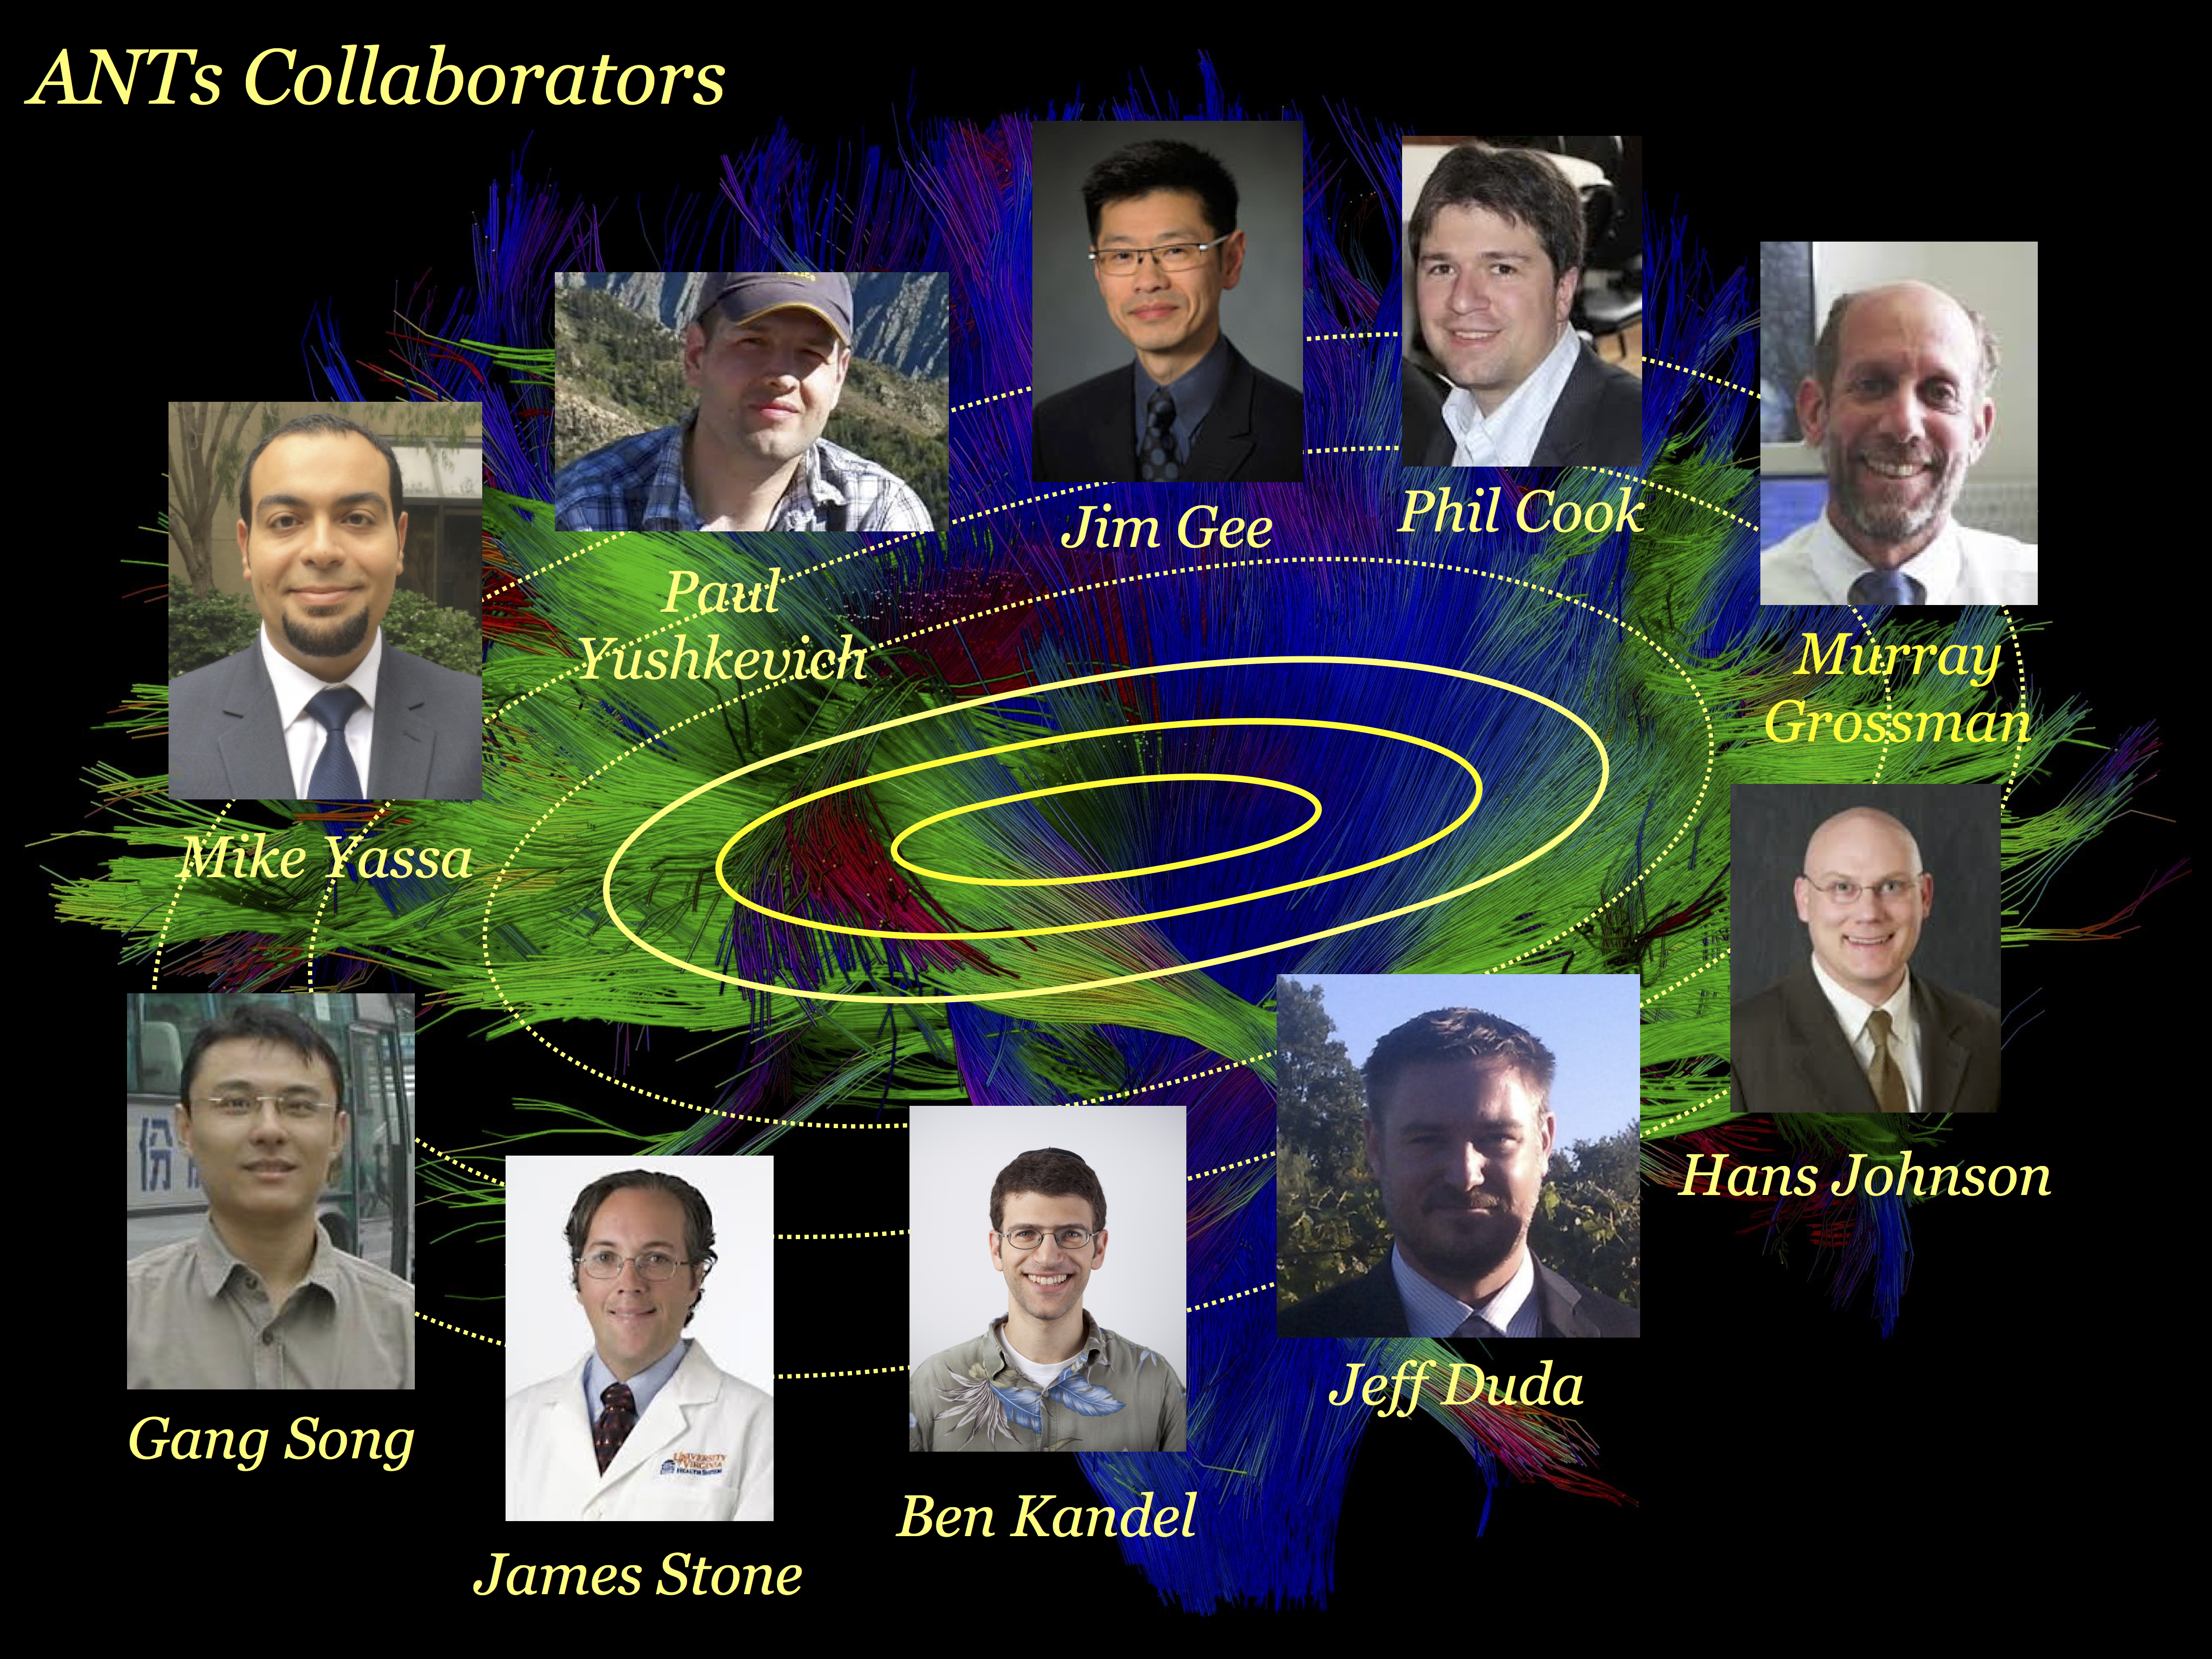
\includegraphics[width=4.75in]{./figures/antsCollaborators2.png}

\end{center}

\(+\) \href{http://neuro.debian.net/pkgs/ants.html}{neurodebian},
\href{http://www.slicer.org/}{slicer},
\href{https://github.com/BRAINSia/BRAINSTools}{brainsfit},
\href{http://nipy.sourceforge.net/nipype/}{nipype},
\href{http://www.itk.org}{itk} and more \ldots{}

\end{frame}

\begin{frame}{Advanced Normalization Tools}

\begin{center}

\includegraphics[width=4.75in]{./tools/figures/coreANtsToolsNeuro.png}

\end{center}

\end{frame}

\begin{frame}{Advanced Normalization Tools \(\rightarrow\) ``ITK-Lung''}

\begin{center}

\includegraphics[width=4.75in]{./tools/figures/coreANtsToolsLung.png}

\end{center}

\end{frame}

\begin{frame}{International competitions}

\begin{itemize}
\item
  \href{http://www.ncbi.nlm.nih.gov/pubmed/19195496}{Klein 2009}: MRI
  brain registration
\item
  \href{http://empire10.isi.uu.nl}{EMPIRE 2010}: CT lung registration
\item
  \href{https://masi.vuse.vanderbilt.edu/workshop2012/index.php/Main_Page}{Multi-Atlas
  Label Challenge 2012}: MRI brain registration and segmentation
\item
  \href{https://masi.vuse.vanderbilt.edu/workshop2013/index.php/MICCAI_2013_SATA_Challenge_and_Workshop:Current_events}{SATA
  Challenge 2013}: MRI cardiac and canine hind leg registration
\item
  \href{http://martinos.org/qtim/miccai2013/}{BRATS 2013}: Multi-modal
  MRI brain segmentation
\item
  \href{http://www.cardiacatlas.org/web/stacom2014/moco-introduction}{STACOM
  2014 MoCo Challenge}: MRI cardiac motion estimation
\end{itemize}

\end{frame}

\begin{frame}{Donoho?}

\centering

\emph{``Papers are just advertisements for the science.''}

\end{frame}

\begin{frame}[fragile]{\texttt{antsRegistration}}

\scriptsize

\begin{Shaded}
\begin{Highlighting}[]
\NormalTok{$ }\ExtensionTok{antsRegistration}\NormalTok{ --help}

\ExtensionTok{COMMAND}\NormalTok{:}
     \ExtensionTok{antsRegistration}
          \ExtensionTok{This}\NormalTok{ program is a user-level registration application meant to utilize}
          \ExtensionTok{ITKv4-only}\NormalTok{ classes. The user can specify any number of }\StringTok{"stages"}\NormalTok{ where a stage}
          \ExtensionTok{consists}\NormalTok{ of a transform}\KeywordTok{;} \ExtensionTok{an}\NormalTok{ image metric}\KeywordTok{;} \ExtensionTok{and}\NormalTok{ iterations, shrink factors, and}
          \ExtensionTok{smoothing}\NormalTok{ sigmas for each level.Note that dimensionality, metric, transform,}
          \ExtensionTok{output}\NormalTok{, convergence, shrink-factors and smoothing-sigmas parameters are}
          \ExtensionTok{mandatory.}

\ExtensionTok{OPTIONS}\NormalTok{:}
     \ExtensionTok{--version}
          \ExtensionTok{Get}\NormalTok{ Version Information.}

     \ExtensionTok{-d}\NormalTok{, --dimensionality 2/3}
          \ExtensionTok{This}\NormalTok{ option forces the image to be treated as a specified-dimensional image. If}
          \ExtensionTok{not}\NormalTok{ specified, we try to infer the dimensionality from the input image.}

     \ExtensionTok{-o}\NormalTok{, --output outputTransformPrefix}
\NormalTok{                  [}\ExtensionTok{outputTransformPrefix}\NormalTok{,}\OperatorTok{<}\NormalTok{outputWarpedImage}\OperatorTok{>}\NormalTok{,}\OperatorTok{<}\NormalTok{outputInverseWarpedImage}\OperatorTok{>}\NormalTok{]}
          \ExtensionTok{Specify}\NormalTok{ the output transform prefix (output format is .nii.gz )}\BuiltInTok{.} \ExtensionTok{Optionally}\NormalTok{, one}
          \ExtensionTok{can}\NormalTok{ choose to warp the moving image to the fixed space and, if the inverse}
          \ExtensionTok{transform}\NormalTok{ exists, one can also output the warped fixed image. Note that only the}
          \ExtensionTok{images}\NormalTok{ specified in the first metric call are warped. Use antsApplyTransforms to}
          \ExtensionTok{warp}\NormalTok{ other images using the resultant transform(s)}\ExtensionTok{.}

     \ExtensionTok{-j}\NormalTok{, --save-state saveSateAsTransform}
          \ExtensionTok{Specify}\NormalTok{ the output file for the current state of the registration. The state}
          \FunctionTok{file}\NormalTok{ is written to an hdf5 composite file. It is specially usefull if we want to}
          \ExtensionTok{save}\NormalTok{ the current state of a SyN registration to the disk, so we can load and}
          \ExtensionTok{restore}\NormalTok{ that later to continue the next registration process directly started}
          \ExtensionTok{from}\NormalTok{ the last saved state. The output file of this flag is the same as the}
          \ExtensionTok{write-composite-transform}\NormalTok{, unless the last transform is a SyN transform. In that}
          \KeywordTok{case}\NormalTok{, the inverse displacement field of the SyN transform is also added to the}
\NormalTok{          output composite transform. Again notice that this file cannot be treated as a}
\NormalTok{          transform, and restore-state option must be used to load the written file by}
\NormalTok{          this flag.}

\NormalTok{     -k, --restore-state restoreStateAsATransform}
\NormalTok{          Specify the initial state of the registration which get immediately used to}
\NormalTok{          directly initialize the registration process. The flag is mutually exclusive}
\NormalTok{          with other intialization flags.If this flag is used, none of the}
\NormalTok{          initial-moving-transform and initial-fixed-transform cannot be used.}

\NormalTok{     -a, --write-composite-transform 1/(0)}
\NormalTok{          Boolean specifying whether or not the composite transform (and its inverse, if}
\NormalTok{          it exists) should be written to an hdf5 composite file. This is false by default}
\NormalTok{          so that only the transform for each stage is written to file.}
\NormalTok{          <VALUES>: 0}

\NormalTok{     -p, --print-similarity-measure-interval <unsignedIntegerValue>}
\NormalTok{          Prints out the CC similarity metric measure between the full-size input fixed}
\NormalTok{          and the transformed moving images at each iteration a value of 0 (the default)}
\NormalTok{          indicates that the full scale computation should not take placeany value greater}
\NormalTok{          than 0 represents the interval of full scale metric computation.}
\NormalTok{          <VALUES>: 0}

\NormalTok{     -v, --write-interval-volumes <unsignedIntegerValue>}
\NormalTok{          Writes out the output volume at each iteration. It helps to present the}
\NormalTok{          registration process as a short movie a value of 0 (the default) indicates that}
\NormalTok{          this option should not take placeany value greater than 0 represents the}
\NormalTok{          interval between the iterations which outputs are written to the disk.}
\NormalTok{          <VALUES>: 0}

\NormalTok{     -z, --collapse-output-transforms (1)/0}
\NormalTok{          Collapse output transforms. Specifically, enabling this option combines all}
\NormalTok{          adjacent transforms wherepossible. All adjacent linear transforms are written to}
\NormalTok{          disk}\KeywordTok{ in}\NormalTok{ the forman itk affine transform }\KeywordTok{(}\NormalTok{called xxxGenericAffine.mat}\KeywordTok{)}\ExtensionTok{.}
          \ExtensionTok{Similarly}\NormalTok{, all adjacent displacement field transforms are combined when written}
          \ExtensionTok{to}\NormalTok{ disk (e.g. xxxWarp.nii.gz and xxxInverseWarp.nii.gz (if available))}\ExtensionTok{.Also}\NormalTok{, an}
          \ExtensionTok{output}\NormalTok{ composite transform including the collapsed transforms is written to the}
          \ExtensionTok{disk}\NormalTok{ (called outputCollapsed(Inverse)}\ExtensionTok{Composite}\NormalTok{)}\ExtensionTok{.}
          \OperatorTok{<}\ExtensionTok{VALUES}\OperatorTok{>}\NormalTok{: 1}

     \ExtensionTok{-i}\NormalTok{, --initialize-transforms-per-stage (1)}\ExtensionTok{/0}
          \ExtensionTok{Initialize}\NormalTok{ linear transforms from the previous stage. By enabling this option,}
          \ExtensionTok{the}\NormalTok{ current linear stage transform is directly intialized from the previous}
          \ExtensionTok{stage}\DataTypeTok{\textbackslash{}'}\NormalTok{s linear transform}\KeywordTok{;} \ExtensionTok{this}\NormalTok{ allows multiple linear stages to be run where}
          \ExtensionTok{each}\NormalTok{ stage directly updates the estimated linear transform from the previous}
          \ExtensionTok{stage.}\NormalTok{ (e.g. Translation -}\OperatorTok{>}\NormalTok{ Rigid -}\OperatorTok{>}\NormalTok{ Affine)}\ExtensionTok{.}
          \OperatorTok{<}\ExtensionTok{VALUES}\OperatorTok{>}\NormalTok{: 0}

     \ExtensionTok{-n}\NormalTok{, --interpolation Linear}
                         \ExtensionTok{NearestNeighbor}
                         \ExtensionTok{MultiLabel}\NormalTok{[}\OperatorTok{<}\NormalTok{sigma=imageSpacing}\OperatorTok{>}\NormalTok{,}\OperatorTok{<}\NormalTok{alpha=4.}\OperatorTok{0>}\NormalTok{]}
                         \ExtensionTok{Gaussian}\NormalTok{[}\OperatorTok{<}\NormalTok{sigma=imageSpacing}\OperatorTok{>}\NormalTok{,}\OperatorTok{<}\NormalTok{alpha=1.}\OperatorTok{0>}\NormalTok{]}
                         \ExtensionTok{BSpline}\NormalTok{[}\OperatorTok{<}\NormalTok{order=}\OperatorTok{3>}\NormalTok{]}
                         \ExtensionTok{CosineWindowedSinc}
                         \ExtensionTok{WelchWindowedSinc}
                         \ExtensionTok{HammingWindowedSinc}
                         \ExtensionTok{LanczosWindowedSinc}
          \ExtensionTok{Several}\NormalTok{ interpolation options are available in ITK. These have all been made}
          \ExtensionTok{available.}\NormalTok{ Currently the interpolator choice is only used to warp (and possibly}
          \ExtensionTok{inverse}\NormalTok{ warp) }\ExtensionTok{the}\NormalTok{ final output image(s)}\ExtensionTok{.}

     \ExtensionTok{-g}\NormalTok{, --restrict-deformation PxQxR}
          \ExtensionTok{This}\NormalTok{ option allows the user to restrict the optimization of the displacement}
          \ExtensionTok{field}\NormalTok{, translation, rigid or affine transform on a per-component basis. For}
          \ExtensionTok{example}\NormalTok{, if one wants to limit the deformation or rotation of 3-D volume to the}
          \ExtensionTok{first}\NormalTok{ two dimensions, this is possible by specifying a weight vector of }\StringTok{'1x1x0'}
          \KeywordTok{for} \ExtensionTok{a}\NormalTok{ deformation field or }\StringTok{'1x1x0x1x1x0'}\NormalTok{ for a rigid}
          \ExtensionTok{transformation.Low-dimensional}\NormalTok{ restriction only works if there are no preceding}
          \ExtensionTok{transformations.}

     \ExtensionTok{-q}\NormalTok{, --initial-fixed-transform initialTransform}
\NormalTok{                                   [}\ExtensionTok{initialTransform}\NormalTok{,}\OperatorTok{<}\NormalTok{useInverse}\OperatorTok{>}\NormalTok{]}
\NormalTok{                                   [}\ExtensionTok{fixedImage}\NormalTok{,movingImage,initializationFeature]}
          \ExtensionTok{Specify}\NormalTok{ the initial fixed transform(s) }\FunctionTok{which}\NormalTok{ get immediately incorporated into}
          \ExtensionTok{the}\NormalTok{ composite transform. The order of the transforms is stack-esque in that the}
          \FunctionTok{last}\NormalTok{ transform specified on the command line is the first to be applied. In}
          \ExtensionTok{addition}\NormalTok{ to initialization with ITK transforms, the user can perform an initial}
          \ExtensionTok{translation}\NormalTok{ alignment by specifying the fixed and moving images and selecting an}
          \ExtensionTok{initialization}\NormalTok{ feature. These features include using the geometric center of the}
          \ExtensionTok{images}\NormalTok{ (=0), }\ExtensionTok{the}\NormalTok{ image intensities (=1), }\ExtensionTok{or}\NormalTok{ the origin of the images (=2)}\ExtensionTok{.}

     \ExtensionTok{-r}\NormalTok{, --initial-moving-transform initialTransform}
\NormalTok{                                    [}\ExtensionTok{initialTransform}\NormalTok{,}\OperatorTok{<}\NormalTok{useInverse}\OperatorTok{>}\NormalTok{]}
\NormalTok{                                    [}\ExtensionTok{fixedImage}\NormalTok{,movingImage,initializationFeature]}
          \ExtensionTok{Specify}\NormalTok{ the initial moving transform(s) }\FunctionTok{which}\NormalTok{ get immediately incorporated into}
          \ExtensionTok{the}\NormalTok{ composite transform. The order of the transforms is stack-esque in that the}
          \FunctionTok{last}\NormalTok{ transform specified on the command line is the first to be applied. In}
          \ExtensionTok{addition}\NormalTok{ to initialization with ITK transforms, the user can perform an initial}
          \ExtensionTok{translation}\NormalTok{ alignment by specifying the fixed and moving images and selecting an}
          \ExtensionTok{initialization}\NormalTok{ feature. These features include using the geometric center of the}
          \ExtensionTok{images}\NormalTok{ (=0), }\ExtensionTok{the}\NormalTok{ image intensities (=1), }\ExtensionTok{or}\NormalTok{ the origin of the images (=2)}\ExtensionTok{.}

     \ExtensionTok{-m}\NormalTok{, --metric CC[fixedImage,movingImage,metricWeight,radius,}\OperatorTok{<}\NormalTok{samplingStrategy=}\DataTypeTok{\{None,Regular,Random\}}\OperatorTok{>}\NormalTok{,}\OperatorTok{<}\NormalTok{samplingPercentage=[0,1]}\OperatorTok{>}\NormalTok{]}
                  \ExtensionTok{MI}\NormalTok{[fixedImage,movingImage,metricWeight,numberOfBins,}\OperatorTok{<}\NormalTok{samplingStrategy=}\DataTypeTok{\{None,Regular,Random\}}\OperatorTok{>}\NormalTok{,}\OperatorTok{<}\NormalTok{samplingPercentage=[0,1]}\OperatorTok{>}\NormalTok{]}
                  \ExtensionTok{Mattes}\NormalTok{[fixedImage,movingImage,metricWeight,numberOfBins,}\OperatorTok{<}\NormalTok{samplingStrategy=}\DataTypeTok{\{None,Regular,Random\}}\OperatorTok{>}\NormalTok{,}\OperatorTok{<}\NormalTok{samplingPercentage=[0,1]}\OperatorTok{>}\NormalTok{]}
                  \ExtensionTok{MeanSquares}\NormalTok{[fixedImage,movingImage,metricWeight,radius=NA,}\OperatorTok{<}\NormalTok{samplingStrategy=}\DataTypeTok{\{None,Regular,Random\}}\OperatorTok{>}\NormalTok{,}\OperatorTok{<}\NormalTok{samplingPercentage=[0,1]}\OperatorTok{>}\NormalTok{]}
                  \ExtensionTok{Demons}\NormalTok{[fixedImage,movingImage,metricWeight,radius=NA,}\OperatorTok{<}\NormalTok{samplingStrategy=}\DataTypeTok{\{None,Regular,Random\}}\OperatorTok{>}\NormalTok{,}\OperatorTok{<}\NormalTok{samplingPercentage=[0,1]}\OperatorTok{>}\NormalTok{]}
                  \ExtensionTok{GC}\NormalTok{[fixedImage,movingImage,metricWeight,radius=NA,}\OperatorTok{<}\NormalTok{samplingStrategy=}\DataTypeTok{\{None,Regular,Random\}}\OperatorTok{>}\NormalTok{,}\OperatorTok{<}\NormalTok{samplingPercentage=[0,1]}\OperatorTok{>}\NormalTok{]}
                  \ExtensionTok{ICP}\NormalTok{[fixedPointSet,movingPointSet,metricWeight,}\OperatorTok{<}\NormalTok{samplingPercentage=[0,1]}\OperatorTok{>}\NormalTok{,}\OperatorTok{<}\NormalTok{boundaryPointsOnly=}\OperatorTok{0>}\NormalTok{]}
                  \ExtensionTok{PSE}\NormalTok{[fixedPointSet,movingPointSet,metricWeight,}\OperatorTok{<}\NormalTok{samplingPercentage=[0,1]}\OperatorTok{>}\NormalTok{,}\OperatorTok{<}\NormalTok{boundaryPointsOnly=}\OperatorTok{0>}\NormalTok{,}\OperatorTok{<}\NormalTok{pointSetSigma=}\OperatorTok{1>}\NormalTok{,}\OperatorTok{<}\NormalTok{kNeighborhood=}\OperatorTok{50>}\NormalTok{]}
                  \ExtensionTok{JHCT}\NormalTok{[fixedPointSet,movingPointSet,metricWeight,}\OperatorTok{<}\NormalTok{samplingPercentage=[0,1]}\OperatorTok{>}\NormalTok{,}\OperatorTok{<}\NormalTok{boundaryPointsOnly=}\OperatorTok{0>}\NormalTok{,}\OperatorTok{<}\NormalTok{pointSetSigma=}\OperatorTok{1>}\NormalTok{,}\OperatorTok{<}\NormalTok{kNeighborhood=}\OperatorTok{50>}\NormalTok{,}\OperatorTok{<}\NormalTok{alpha=1.}\OperatorTok{1>}\NormalTok{,}\OperatorTok{<}\NormalTok{useAnisotropicCovariances=}\OperatorTok{1>}\NormalTok{]}
                  \ExtensionTok{IGDM}\NormalTok{[fixedImage,movingImage,metricWeight,fixedMask,movingMask,}\OperatorTok{<}\NormalTok{neighborhoodRadius=0x0}\OperatorTok{>}\NormalTok{,}\OperatorTok{<}\NormalTok{intensitySigma=}\OperatorTok{0>}\NormalTok{,}\OperatorTok{<}\NormalTok{distanceSigma=}\OperatorTok{0>}\NormalTok{,}\OperatorTok{<}\NormalTok{kNeighborhood=}\OperatorTok{1>}\NormalTok{,}\OperatorTok{<}\NormalTok{gradientSigma=}\OperatorTok{1>}\NormalTok{]}
          \ExtensionTok{These}\NormalTok{ image metrics are available--- CC: ANTS neighborhood cross correlation,}
          \ExtensionTok{MI}\NormalTok{: Mutual information, Demons: (Thirion), }\ExtensionTok{MeanSquares}\NormalTok{, and GC: Global}
          \ExtensionTok{Correlation.}\NormalTok{ The }\StringTok{"metricWeight"}\NormalTok{ variable is used to modulate the per stage}
          \ExtensionTok{weighting}\NormalTok{ of the metrics. The metrics can also employ a sampling strategy}
          \ExtensionTok{defined}\NormalTok{ by a sampling percentage. The sampling strategy defaults to }\StringTok{'None'}\NormalTok{ (aka}
          \ExtensionTok{a}\NormalTok{ dense sampling of one sample per voxel), }\ExtensionTok{otherwise}\NormalTok{ it defines a point set over}
          \FunctionTok{which}\NormalTok{ to optimize the metric. The point set can be on a regular lattice or a}
          \ExtensionTok{random}\NormalTok{ lattice of points slightly perturbed to minimize aliasing artifacts.}
          \ExtensionTok{samplingPercentage}\NormalTok{ defines the fraction of points to select from the domain. In}
          \ExtensionTok{addition}\NormalTok{, three point set metrics are available: Euclidean (ICP), }\ExtensionTok{Point-set}
          \ExtensionTok{expectation}\NormalTok{ (PSE), }\ExtensionTok{and}\NormalTok{ Jensen-Havrda-Charvet-Tsallis (JHCT)}\ExtensionTok{.}

     \ExtensionTok{-t}\NormalTok{, --transform Rigid[gradientStep]}
                     \ExtensionTok{Affine}\NormalTok{[gradientStep]}
                     \ExtensionTok{CompositeAffine}\NormalTok{[gradientStep]}
                     \ExtensionTok{Similarity}\NormalTok{[gradientStep]}
                     \ExtensionTok{Translation}\NormalTok{[gradientStep]}
                     \ExtensionTok{BSpline}\NormalTok{[gradientStep,meshSizeAtBaseLevel]}
                     \ExtensionTok{GaussianDisplacementField}\NormalTok{[gradientStep,updateFieldVarianceInVoxelSpace,totalFieldVarianceInVoxelSpace]}
                     \ExtensionTok{BSplineDisplacementField}\NormalTok{[gradientStep,updateFieldMeshSizeAtBaseLevel,totalFieldMeshSizeAtBaseLevel,}\OperatorTok{<}\NormalTok{splineOrder=}\OperatorTok{3>}\NormalTok{]}
                     \ExtensionTok{TimeVaryingVelocityField}\NormalTok{[gradientStep,numberOfTimeIndices,updateFieldVarianceInVoxelSpace,updateFieldTimeVariance,totalFieldVarianceInVoxelSpace,totalFieldTimeVariance]}
                     \ExtensionTok{TimeVaryingBSplineVelocityField}\NormalTok{[gradientStep,velocityFieldMeshSize,}\OperatorTok{<}\NormalTok{numberOfTimePointSamples=}\OperatorTok{4>}\NormalTok{,}\OperatorTok{<}\NormalTok{splineOrder=}\OperatorTok{3>}\NormalTok{]}
                     \ExtensionTok{SyN}\NormalTok{[gradientStep,updateFieldVarianceInVoxelSpace,totalFieldVarianceInVoxelSpace]}
                     \ExtensionTok{BSplineSyN}\NormalTok{[gradientStep,updateFieldMeshSizeAtBaseLevel,totalFieldMeshSizeAtBaseLevel,}\OperatorTok{<}\NormalTok{splineOrder=}\OperatorTok{3>}\NormalTok{]}
                     \ExtensionTok{Exponential}\NormalTok{[gradientStep,updateFieldVarianceInVoxelSpace,velocityFieldVarianceInVoxelSpace,}\OperatorTok{<}\NormalTok{numberOfIntegrationSteps}\OperatorTok{>}\NormalTok{]}
                     \ExtensionTok{BSplineExponential}\NormalTok{[gradientStep,updateFieldMeshSizeAtBaseLevel,velocityFieldMeshSizeAtBaseLevel,}\OperatorTok{<}\NormalTok{numberOfIntegrationSteps}\OperatorTok{>}\NormalTok{,}\OperatorTok{<}\NormalTok{splineOrder=}\OperatorTok{3>}\NormalTok{]}
          \ExtensionTok{Several}\NormalTok{ transform options are available. The gradientStep or learningRate}
          \ExtensionTok{characterizes}\NormalTok{ the gradient descent optimization and is scaled appropriately for}
          \ExtensionTok{each}\NormalTok{ transform using the shift scales estimator. Subsequent parameters are}
          \ExtensionTok{transform-specific}\NormalTok{ and can be determined from the usage. For the B-spline}
          \ExtensionTok{transforms}\NormalTok{ one can also specify the smoothing in terms of spline distance (i.e.}
          \ExtensionTok{knot}\NormalTok{ spacing)}\ExtensionTok{.}

     \ExtensionTok{-c}\NormalTok{, --convergence MxNxO}
\NormalTok{                       [}\ExtensionTok{MxNxO}\NormalTok{,}\OperatorTok{<}\NormalTok{convergenceThreshold=1e-}\OperatorTok{6>}\NormalTok{,}\OperatorTok{<}\NormalTok{convergenceWindowSize=}\OperatorTok{10>}\NormalTok{]}
          \ExtensionTok{Convergence}\NormalTok{ is determined from the number of iterations per level and is}
          \ExtensionTok{determined}\NormalTok{ by fitting a line to the normalized energy profile of the last N}
          \ExtensionTok{iterations}\NormalTok{ (where N is specified by the window size) }\ExtensionTok{and}\NormalTok{ determining the slope}
          \FunctionTok{which}\NormalTok{ is then compared with the convergence threshold.}

     \ExtensionTok{-s}\NormalTok{, --smoothing-sigmas MxNxO...}
          \ExtensionTok{Specify}\NormalTok{ the sigma of gaussian smoothing at each level. Units are given in terms}
          \ExtensionTok{of}\NormalTok{ voxels (}\StringTok{'vox'}\NormalTok{) }\ExtensionTok{or}\NormalTok{ physical spacing (}\StringTok{'mm'}\NormalTok{)}\BuiltInTok{.} \ExtensionTok{Example}\NormalTok{ usage is }\StringTok{'4x2x1mm'}\NormalTok{ and}
          \StringTok{'4x2x1vox'} \ExtensionTok{where}\NormalTok{ no units implies voxel spacing.}

     \ExtensionTok{-f}\NormalTok{, --shrink-factors MxNxO...}
          \ExtensionTok{Specify}\NormalTok{ the shrink factor for the virtual domain (typically the fixed image) }\ExtensionTok{at}
          \ExtensionTok{each}\NormalTok{ level.}

     \ExtensionTok{-u}\NormalTok{, --use-histogram-matching}
          \ExtensionTok{Histogram}\NormalTok{ match the images before registration.}

     \ExtensionTok{-l}\NormalTok{, --use-estimate-learning-rate-once}
          \ExtensionTok{turn}\NormalTok{ on the option that lets you estimate the learning rate step size only at}
          \ExtensionTok{the}\NormalTok{ beginning of each level. * useful as a second stage of fine-scale}
          \ExtensionTok{registration.}

     \ExtensionTok{-w}\NormalTok{, --winsorize-image-intensities [lowerQuantile,upperQuantile]}
          \ExtensionTok{Winsorize}\NormalTok{ data based on specified quantiles.}

     \ExtensionTok{-x}\NormalTok{, --masks [fixedImageMask,movingImageMask]}
          \ExtensionTok{Image}\NormalTok{ masks to limit voxels considered by the metric.}

     \ExtensionTok{--float}
          \ExtensionTok{Use} \StringTok{'float'}\NormalTok{ instead of }\StringTok{'double'}\NormalTok{ for computations.}
          \OperatorTok{<}\ExtensionTok{VALUES}\OperatorTok{>}\NormalTok{: 0}

     \ExtensionTok{-v}\NormalTok{, --verbose (0)}\ExtensionTok{/1}
          \ExtensionTok{Verbose}\NormalTok{ output.}

     \ExtensionTok{-h}
          \ExtensionTok{Print}\NormalTok{ the help menu (short version)}\ExtensionTok{.}

     \ExtensionTok{--help}
          \ExtensionTok{Print}\NormalTok{ the help menu. Will also print values used on the current command line}
          \ExtensionTok{call.}
\end{Highlighting}
\end{Shaded}

\end{frame}

\section{Putting it all together---the ANTs cortical thickness
pipeline}\label{putting-it-all-togetherthe-ants-cortical-thickness-pipeline}

\begin{frame}{Cortical thickness studies}

\scriptsize

\begin{longtable}[]{@{}ll@{}}
\toprule
Column1 & Column2\tabularnewline
\midrule
\endhead
Tetris-playing ability & chronic pancreatitis\tabularnewline
Huntington's disease & obsessive-compulsive disorder\tabularnewline
schizophrenia & ADHD\tabularnewline
bipolar disorder & obesity\tabularnewline
Alzheimer's disease & heritable depression\tabularnewline
frontotemporal dementia & elderly depression\tabularnewline
Parkinson's disease & age\tabularnewline
Williams syndrome & gender\tabularnewline
multiple sclerosis & handedness\tabularnewline
autism & intelligence\tabularnewline
migraines & athletic ability\tabularnewline
chronic smoking & meditative practices\tabularnewline
alcoholism & musical ability\tabularnewline
cocaine addiction & tendency toward criminality\tabularnewline
Tourette syndrome in children & childhood sexual abuse in female
adolescents\tabularnewline
scoliosis in female adolescents & traumatic brain injury\tabularnewline
early-onset blindness & untreated male-to-female
transsexuality\tabularnewline
\bottomrule
\end{longtable}

\end{frame}

\begin{frame}{The ANTs structural brain mapping workflow}

\begin{centering}

\includegraphics[width=4.5in]{./evaluation/figures/pipeline.png}

\end{centering}

\end{frame}

\begin{frame}{Template building}

\emph{Tailor data to your specific cohort}

\begin{centering}

\includegraphics[width=3in]{./evaluation/figures/templates.png}

\end{centering}

\small

\begin{itemize}
\tightlist
\item
  Templates representing the average mean shape and intensity are built
  directly from the cohort to be analyzed, e.g.~pediatric
  vs.~middle-aged brains.\\
\item
  Acquisition and anonymization (e.g.~defacing) protocols are often
  different.
\end{itemize}

\end{frame}

\begin{frame}{Template priors}

\begin{centering}

\includegraphics[width=2.5in]{./evaluation/figures/templatePriors.png}

\end{centering}

\small

Each template is
\href{https://github.com/ntustison/antsCookTemplatePriorsExample}{processed}
to produce auxiliary images which are used for brain extraction and
brain segmentation.

\end{frame}

\begin{frame}{Brain extraction comparison}

\begin{centering}

\includegraphics[width=3.5in]{./evaluation/figures/brainExtraction.png}

\end{centering}

\small

Comparison with de facto standard FreeSurfer package. Note the
difference in separation of the gray matter from the surrounding CSF. (0
failures out of 1205 scans)

\end{frame}

\begin{frame}[fragile]{Brain segmentation}

\begin{centering}

\includegraphics[width=3.5in]{./evaluation/figures/brainSegmentation.png}

\end{centering}

\small

Randomly selected healthy individuals. \texttt{Atropos} gets good
performance across ages.

\end{frame}

\begin{frame}{Cortical thickness maps}

\begin{centering}

\includegraphics[width=4in]{./evaluation/figures/corticalThicknessEstimation.png}

\end{centering}

\small

In contrast to FreeSurfer which warps coupled surface meshes to segment
the gray matter, \emph{ANTs} diffeomorphically registers the white
matter to the combined gray/white matters while simultaneously
estimating thickness.

\end{frame}

\begin{frame}

\begin{centering}

\Large

{\bf But without ground truth, how does one evaluate the pipeline?}

\end{centering}

\end{frame}

\begin{frame}{Predict age and gender}

\begin{centering}

$AGE \sim VOLUME + GENDER + \sum_{i=1}^{62} T(DKT_i)$

\end{centering}

\end{frame}

\begin{frame}{Prediction from cortical thickness data}

\begin{centering}

\includegraphics[width=4in]{./evaluation/figures/evaluation.png}

\end{centering}

\end{frame}

\begin{frame}{Regional importance comparison}

\begin{centering}

\small
ANTs (left) vs. FreeSurfer (right)

\includegraphics[width=4in]{./evaluation/figures/antsvfreesurfer_Importance.png}

\end{centering}

\end{frame}

\begin{frame}{Regional measurements}

\begin{centering}

\includegraphics[width=4in]{./evaluation/figures/antsvfreesurfer_regionalPlots.png}

\end{centering}

\end{frame}

\begin{frame}{Longitudinal processing}

\includegraphics{./longitudinal/figures/longitudinalPipeline.png}

\end{frame}

\section{Advanced Normalization Tools in R
(ANTsR)}\label{advanced-normalization-tools-in-r-antsr}

\begin{frame}{Multimodal Brain Tumor Segmentation (BRATS 2013)}

\begin{centering}

\includegraphics[width=4.5in]{./competitions/figures/brats2013results1.png}

\end{centering}

\small

\href{http://www.ncbi.nlm.nih.gov/pubmed/25433513}{Tustison, et al.,
Optimal symmetric multimodal templates and concatenated random forests
for supervised brain tumor segmentation (simplified) with \emph{ANTsR},
\emph{Neuroinformatics}.}

\end{frame}

\begin{frame}{White matter hyperintensities in TBI}

\begin{centering}

\includegraphics[width=4.5in]{./wmhs/figures/wmhPipeline.png}

\end{centering}

\end{frame}

\begin{frame}{Social behavior and immunity dysfunction in mice}

\begin{centering}

\includegraphics[width=3in]{./antsr/figures/filiano_rsfmri.png}

\end{centering}

\end{frame}

\begin{frame}{Other ANTsR work}

\begin{itemize}
\item
  \href{http://www.nature.com/articles/sdata20153}{Pediatric template of
  brain perfusion}
\item
  \href{http://www.ncbi.nlm.nih.gov/pubmed/26756101}{Automated
  segmentation of chronic stroke lesions using LINDA: Lesion
  identification with neighborhood data analysis}
\item
  \href{http://www.ncbi.nlm.nih.gov/pubmed/25448483}{Eigenanatomy}
\item
  \href{https://github.com/stnava/ANTsRNet}{ANTsRNet}: a growing
  collection of popular deep learning architectures
\end{itemize}

\end{frame}

\begin{frame}{Open source}

\begin{itemize}
\item
  \url{https://github.com/stnava/ANTs}
\item
  \url{https://github.com/stnava/ANTsR}
\item
  \url{https://github.com/stnava/ANTsRNet}
\end{itemize}

\end{frame}

\end{document}
